\section{Effect and Propagation of Systematic Uncertainties}
%{\it Assigned to:} {\bf Chris Marshall} with contributions by Luke Pickering and Callum Wilkinson. 
\label{sec:physics-lbnosc-syst}
Content will include: 
\begin{itemize}
    \item Overview of the systematic uncertainties
    \item Discussion of cancellations and constraints
    \item Discussion of what has the largest impacts on sensitivities
    \item Potential sources of bias
\end{itemize}

%\subsubsection{Uncertainties \& Constraint Requirements from ND Analyses}
Potential figures and tables include: 
\begin{itemize}
\item Error envelopes (vs energy) pre and post ND constraints (New plot)
\item CafAna response functions examples 
\item CafAna chisq vs paramater constraint examples 
\item Table: Parameter constraints with pre/post fit $1\sigma$ uncertainties per systematic (New)
\item Covariance matrix 
\item (Placeholder added) Example DUNE PRISM style prediction with representative cancellation of uncertainties.
\item (Placeholder added) Missing proton energy fake data study bias demonstration and resolution.
\end{itemize}

Systematic uncertainties can be broadly divided into three categories: flux, neutrino interactions, and detector effects. Flux uncertainties are described in Section~\ref{sec:nu-osc-05}. Neutrino cross section uncertainties are described in Section~\ref{sec:nu-osc-05}. Detector-related uncertainties are discussed for the near detector in Section~\ref{sec:nu-osc-06}, and for the far detector in Section~\ref{sec:nu-osc-07}. This section will cover the ways in which uncertainties are constrained in the near-far oscillation fit, and the individual uncertainties with the largest impact on oscillation parameter sensitivities.

\fixme{The near-far fit is an ongoing effort. We do not currently have any results with the full suite of systematics. This section will be written later.}

\subsection{Systematic uncertainty constraints and cancellations}

The near detector samples provide constraints on flux and cross section uncertainties.

\fixme{Pre- and Post-fit error matrices}

\fixme{Placeholder plot added for DUNE PRISM built spectra. Will discuss with DUNE PRISM group Thursday to understand best surrounding text}

\begin{figure}
  \centering
  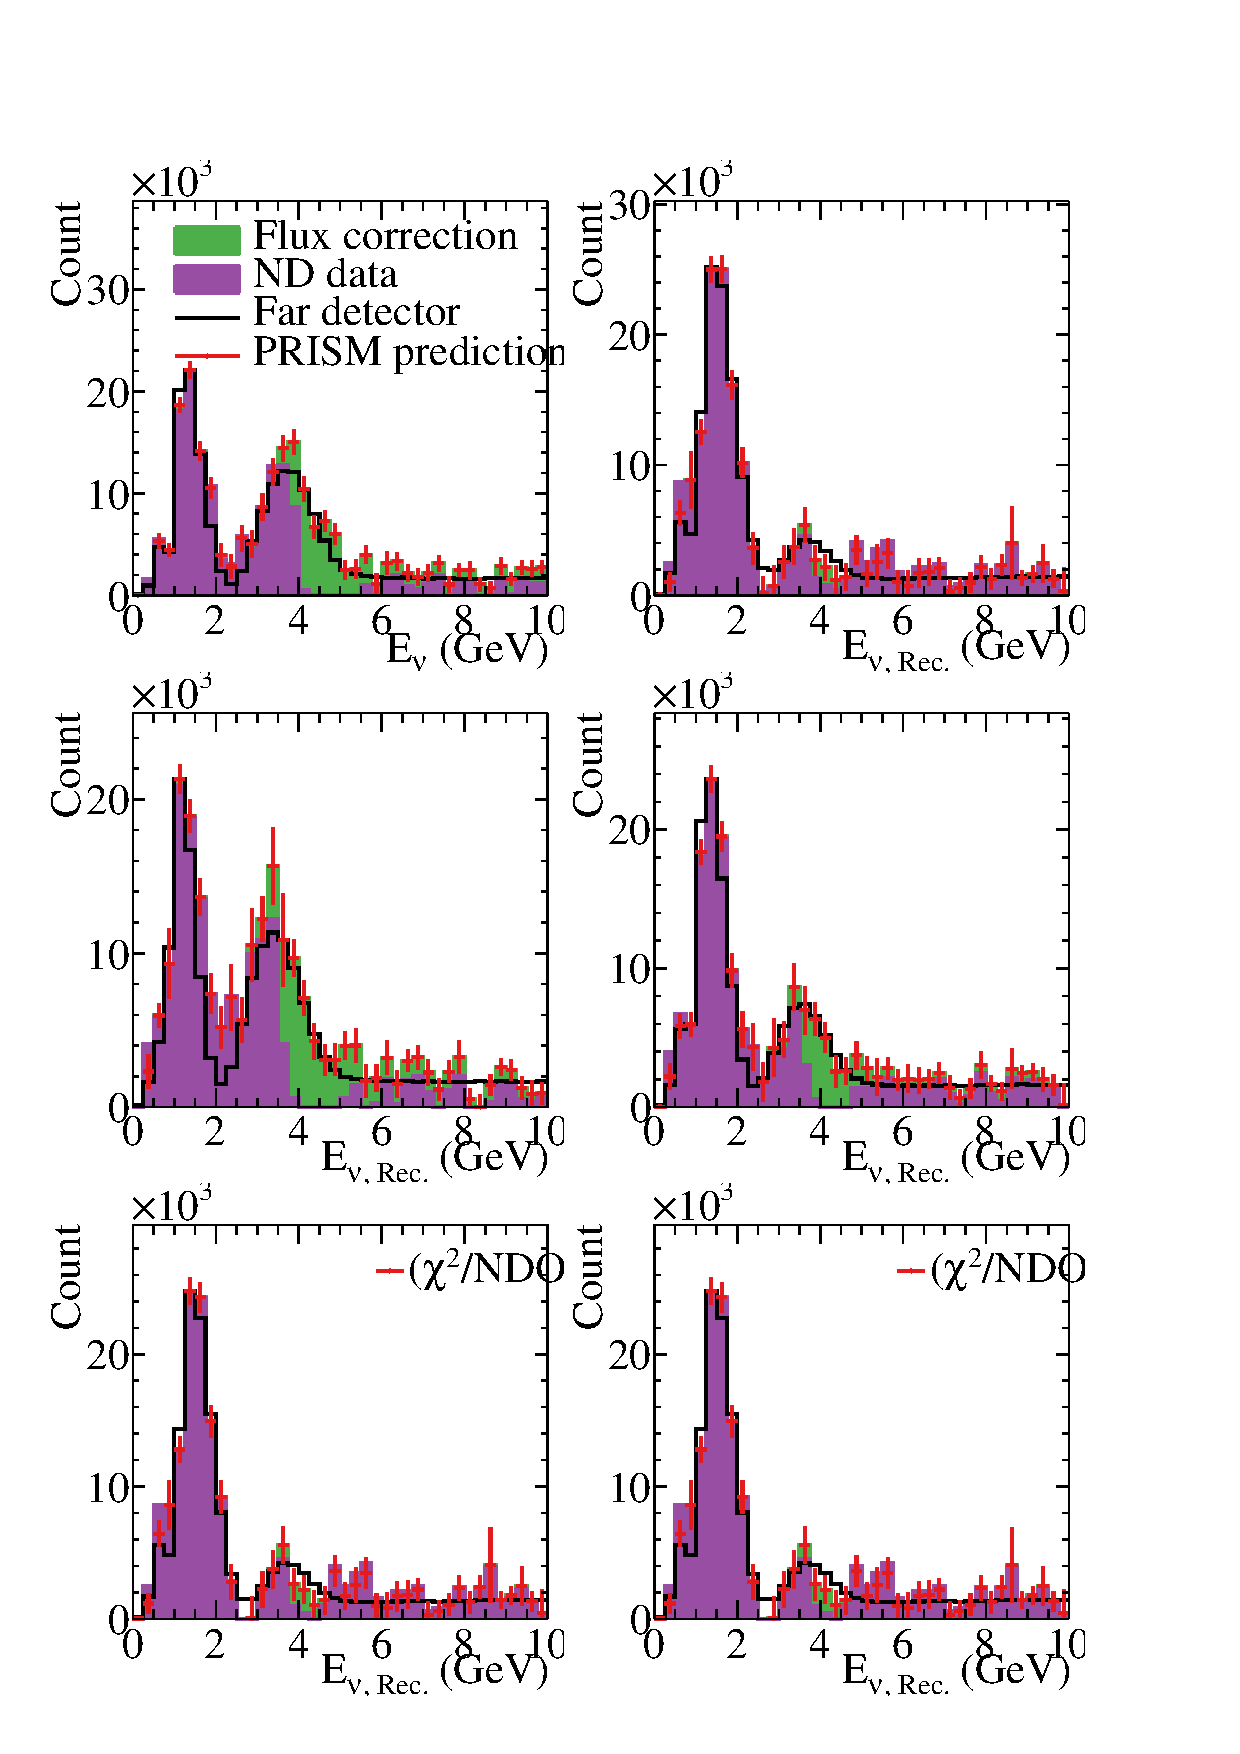
\includegraphics[width=10cm]{graphics/PRISMPrediction_Scan.pdf}
  \caption{The full far detector prediction built from corrected linear combinations of near detector `observables'. This is shown for the $4\,\textrm{m}$ (\emph{top}) and $7\,\textrm{m}$ (\emph{bottom}) wide detectors and projected into true neutrino energy (\emph{left}) and reconstructed neutrino energy (\emph{right}). The correspondence between far detector prediction and observation can be seen to be better for the $7\,\textrm{m}$ wide detector, where the efficiency correction is less aggressive. }
  \label{fig:PRISM_PRISMPrediction}
\end{figure}

\subsection{Largest post-fit systematic uncertainties}

Near detector data does not fully cancel systematic effects.
\fixme{List the largest few uncertainties}
\fixme{anticorrelations between flux and XS}

\subsection{Avoiding bias}

\begin{figure}[h]
\centering
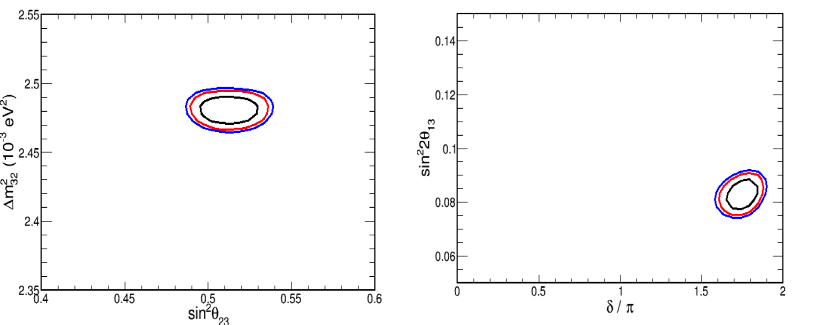
\includegraphics[angle=0,width=16cm,height=5.6cm]{graphics/protonEbias_fluxfloated.png}
\caption{Contours of fitting 20\% missing proton energy fake data for true oscillated parameters corresponding to  sin$^{2}\theta_{23}$=0.5, $\Delta$m$^{2}_{23}$=2.45x10$^{-3}$ eV$^{2}$, $\Delta$=1.5$\pi$ and sin$^{2}2\theta_{13}$=0.085. Nuisance parameters corresponding the flux allowed to float.
Left: sin$^{2}\theta_{23}$ vs. $\Delta$m$^{2}_{32}$ Right: $\delta$ vs. sin$^{2}2\theta_{13}$) planes with flux constraints.} \label{protonFDSbias}
\end{figure}
\fixme{Stars need to be added to the plot to indicate the true values of the parameters}

Figure~\ref{protonFDSbias} shows how measurements of oscillation may be biased due to mis-modelling in the interaction model. This specific mock data, described in Section~\ref{sec:nu-osc-05}, is a plausible modification to the reconstructed-true energy association. Furthermore, the underlying cross section model issue is not visible with only the on-axis event sample, as shown in Fig~\ref{fig:protonFDS_spectra1}. However, off-axis samples show disagreement with the on-axis-only ND fit; off-axis samples may be used to diagnose and resolve underlying interaction mis-modelling~\ref{fig:protonFDS_spectra2}. %\fixme{Mike: please read and expand/adjust}


\begin{figure}[h]
\centering
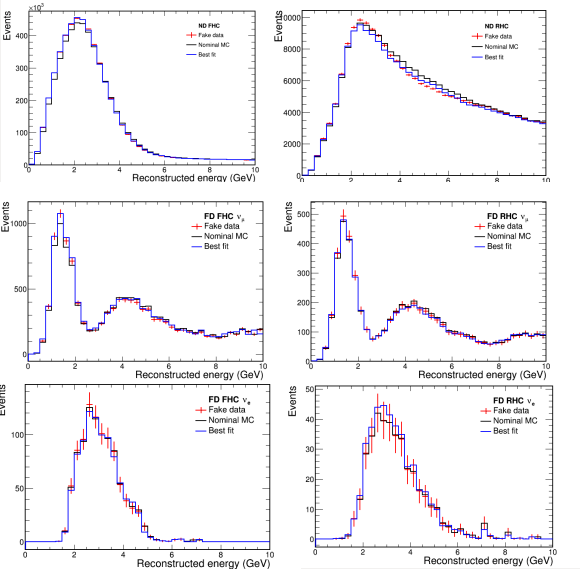
\includegraphics[angle=0,width=16cm,height=15.6cm]{graphics/protonFDS_spectra1.png}
\caption{20\% missing proton energy fake data fitting spectra for ND and FD FHC and RHC with flux constraints. The black spectra are nominal, the red are fake data and the blue are best fit.}
\label{fig:protonFDS_spectra1}
\end{figure}

\begin{figure}[h]
\centering
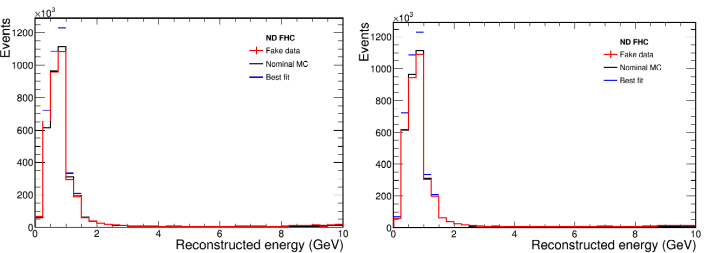
\includegraphics[angle=0,width=16cm,height=5.6cm]{graphics/protonFDS_spectra2.png}
\caption{With flux parameters, comparison of on-axis best fit(blue), 30 m off-axis nominal(black) and 30 m off-axis fake data(red) spectra. Left: FHC; Right: RHC. }
\label{fig:protonFDS_spectra2}
\end{figure}
\fixme{The oscillated fake data spectra can be removed here to save space}